% Dokumentinformationen
\title{Applied Electromagnetics}
\author{HSR-Stud R. Christen }
%\version{$Revision: Marie $ - powered by \LaTeX}
\documentclass[8spt,twoside,a4paper,fleqn]{article}

% Header
%%%%%%%%%%%%%%%%%%%%%%%%%%%%%%%%%%%%%%%
%% Makros & anderer Low-Level bastel %%
%%%%%%%%%%%%%%%%%%%%%%%%%%%%%%%%%%%%%%%
\makeatletter
%% Makros für Titel, Autor und Datum 
%% Dank diesem Makro stehen Titel, Autor und Datum überall im Dokument zur verfügung
%% Date hat zudem den Default-Wert \today
\def\@Title{}
\def\@Author{}
\def\@Date{\today}
\newcommand{\Title}{\@Title}
\newcommand{\Author}{\@Author}
\newcommand{\Date}{\@Date}
\AtBeginDocument{%
  \let\@Title\@title
  \let\@Author\@author
  \let\@Date\@date
}

%% Makros für den Arraystretch (bei uns meist in Tabellen genutzt, welche Formeln enthalten)
% Default Value
\def\@ArrayStretchDefault{1} % Entspricht der Voreinstellung von Latex

% Setzt einen neuen Wert für den arraystretch
\newcommand{\setArrayStretch}[1]{\renewcommand{\arraystretch}{#1}}

% Setzt den arraystretch zurück auf den default wert
\newcommand{\resetArrayStretch}{\renewcommand{\arraystretch}{\@ArrayStretchDefault}}

% Makro zum setzten des Default arraystretch. Kann nur in der Präambel verwendet werden.
\newcommand{\setDefaultArrayStretch}[1]{%
	\AtBeginDocument{%
		\def\@ArrayStretchDefault{#1}
		\renewcommand{\arraystretch}{#1}
	}
}
\makeatother


%%%%%%%%%%%%%%%%%%%%%%%
%% Wichtige Packages %%
%%%%%%%%%%%%%%%%%%%%%%%
\usepackage[utf8]{inputenc} % UTF-8 unterstützung
\usepackage[english, ngerman]{babel} % Silbentrennung
\usepackage[automark]{scrpage2} % Header und Footer
\usepackage{tabularx}

% Für Abbildungen mit mehreren kleinen Bilder
% Doku: http://www.ctan.org/tex-archive/macros/latex/contrib/caption/
\usepackage{caption}
\usepackage{subcaption}

\ifx \GUARDhsrColors \undefined
\def\GUARDhsrColors{}

\usepackage[table]{xcolor}

\definecolor{HSRWhite}{cmyk}{0,0,0,0}

\definecolor{HSRBlue}{cmyk}{1,0.4,0,0.2}
\definecolor{HSRBlue80}{cmyk}{0.8,0.32,0,0.16}
\definecolor{HSRBlue60}{cmyk}{0.6,0.24,0,0.12}
\definecolor{HSRBlue40}{cmyk}{0.4,0.16,0,0.08}
\definecolor{HSRBlue20}{cmyk}{0.2,0.08,0,0.04}

\definecolor{HSRLightGray}{cmyk}{0,0,0,0.30}
\definecolor{HSRLightGray80}{cmyk}{0,0,0,0.24}
\definecolor{HSRLightGray60}{cmyk}{0,0,0,0.18}
\definecolor{HSRLightGray40}{cmyk}{0,0,0,0.12}
\definecolor{HSRLightGray20}{cmyk}{0,0,0,0.06}

\definecolor{HSRSchwarz}{cmyk}{0,0,0,1}
\definecolor{HSRSchwarz80}{cmyk}{0,0,0,0.8}
\definecolor{HSRSchwarz60}{cmyk}{0,0,0,0.6}
\definecolor{HSRSchwarz40}{cmyk}{0,0,0,0.4}
\definecolor{HSRSchwarz20}{cmyk}{0,0,0,0.2}

\definecolor{HSRHematite}{cmyk}{0.6,1,0.4,0.2}
\definecolor{HSRHematite80}{cmyk}{0.48,0.80,0.32,0.16}
\definecolor{HSRHematite60}{cmyk}{0.36,0.60,0.24,0.12}
\definecolor{HSRHematite40}{cmyk}{0.24,0.40,0.16,0.08}
\definecolor{HSRHematite20}{cmyk}{0.12,0.20,0.08,0.04}

\definecolor{HSRLakeGreen}{cmyk}{0.70,0.30,0.45,0.05}
\definecolor{HSRLakeGreen80}{cmyk}{0.56,0.24,0.36,0.03}
\definecolor{HSRLakeGreen60}{cmyk}{0.42,0.18,0.27,0.02}
\definecolor{HSRLakeGreen40}{cmyk}{0.28,0.06,0.13,0.06}
\definecolor{HSRLakeGreen20}{cmyk}{0.14,0.06,0.09,0.01}

\definecolor{HSRReed}{cmyk}{0.10,0.25,0.45,0.60}
\definecolor{HSRReed80}{cmyk}{0.08,0.20,0.36,0.48}
\definecolor{HSRReed60}{cmyk}{0.06,0.15,0.27,0.36}
\definecolor{HSRReed40}{cmyk}{0.04,0.10,0.18,0.24}
\definecolor{HSRReed20}{cmyk}{0.02,0.05,0.09,0.12}

\definecolor{HSRPetrol}{cmyk}{1,0.18,0,0.45}
\definecolor{HSRPetrol80}{cmyk}{0.64,0.08,0.12,0.32}
\definecolor{HSRPetrol60}{cmyk}{0.48,0.06,0.09,0.24}
\definecolor{HSRPetrol40}{cmyk}{0.32,0.04,0.06,0.16}
\definecolor{HSRPetrol20}{cmyk}{0.16,0.02,0.03,0.08}

\definecolor{HSRBasswood}{cmyk}{0.25,0.05,0.70,0.15}
\definecolor{HSRBasswood80}{cmyk}{0.20,0.04,0.56,0.12}
\definecolor{HSRBasswood60}{cmyk}{0.15,0.03,0.42,0.09}
\definecolor{HSRBasswood40}{cmyk}{0.10,0.02,0.28,0.06}
\definecolor{HSRBasswood20}{cmyk}{0.05,0.01,0.14,0.03}


\fi
\ifx\GUARDmathe\undefined
\def\GUARDmathe{}

\usepackage{amssymb}
% Das mathtools package ist eine Erweiterung zum amsmath package.
% Das amsmath package wird dabei automatisch geladen
\usepackage{mathtools}


% Package mit vielen weiteren Mathe Symbolen
% http://www.ctan.org/tex-archive/fonts/mathabx
\usepackage{mathabx}

% This package defines commands to access bold math symbols. The basic command
% is \bm which may be used to make the math expression in its argument be typeset
% using bold fonts.
\usepackage{bm}

\fi
\ifx\GUARDenumitem\undefined
\def\GUARDenumitem{}

\usepackage{enumitem}

\fi

% Seitenränder für Formelsammlungen
\usepackage[left=1cm,right=1cm,top=1cm,bottom=1cm,includeheadfoot]{geometry}

\usepackage{multirow} % Create tabular cells spanning multiple rows
\usepackage{multicol} % In­ter­mix sin­gle and mul­ti­ple columns
\usepackage{rotating} % Rotation tools, including rotated fullpage floats


%%%%%%%%%%%%%%%%%%%%%%%%%%%%%%%%%%%
%% Layout der Kopf und Fusszeile %%
%%%%%%%%%%%%%%%%%%%%%%%%%%%%%%%%%%%
\deftripstyle{zusammenfassung}[0pt][0.5pt]
	{\Title}	% Kopfzeile innen
	{\headmark}	% Kopfzeile mitte
	{\pagemark}	% Kopfzeile aussen
	{\Author}	% Fusszeile innen
	{
\includegraphics[width=1.6cm]{./header/lizenzen/cc-by-nc-sa/small.png}}			% Fusszeile mitte
	{\Date}	% Fusszeile aussen
\pagestyle{zusammenfassung}



% Makros für Verweise auf ein Buch oder Skript
\newcommand{\buch}[1]{\texorpdfstring{$_{\textcolor{HSRLakeGreen}{\mbox{\small{#1}}}}$}{}}
\newcommand{\buchSeite}[1]{\texorpdfstring{\ensuremath{_{\textcolor{red}{\mbox{\small{ S#1}}}}}}{}}
\newcommand{\skript}[1]{\texorpdfstring{$_{\textcolor{HSRReed}{\mbox{\small{#1}}}}$}{}}
\newcommand{\formelbuch}[1]{$_{\textcolor{red}{\mbox{\small{S#1}}}}$}

% Zeilenhöhe Tabellen:
\newcommand{\arraystretchOriginal}{1.5}
\renewcommand{\arraystretch}{\arraystretchOriginal}

\setlength{\parindent}{0pt}
\usepackage{tikz}
\usepackage{textcomp, pxfonts, enumitem}
\usetikzlibrary{intersections}
\usepackage{longtable}
\usetikzlibrary{calc}
\usetikzlibrary{through}

\usepackage{adjustbox}
\usepackage{caption}
\usepackage{graphicx}
\usepackage{subcaption}
% Setzt ein zentriertes Bild mit Beschriftung
% Syntax: \abb{Pfad zum Bild}{Bildgrösse}{Beschriftung des Bildes}
\newcounter{abbildungen} \stepcounter{abbildungen}
\newcommand{\abb}[3]{
\begin{center}
\includegraphics[width=#2]{#1} \\
Abbildung \arabic{abbildungen}: #3
\stepcounter{abbildungen}
    \end{center}
}

% Document
\begin{document}
\section{Fundamentals}

\begin{tabular}{|l|c|c|}
\hline \textbf{Description} & \textbf{Symbol} & \textbf{Unit} \\ 
\hline Free electric charge in the system & $Q$ & $C = As$ \\
\hline Volumetric free charge density & $\rho$ & $\frac{C}{m^3}$ \\
\hline Individual electric current flowing through the surface $S$ & $I_i$ & $A$ \\
\hline Magnetic flux through the surface $S$ & $\Phi$	& $Wb = Tm^2$\\
\hline Induced voltage along the closed loop $\delta S$ & $u_i$ & $V$ \\
\hline Electric current density & $\vec{J} = \sigma \vec{E}$ & $\frac{A}{m^2}$\\
\hline Electric flux density & $\vec{D} = \varepsilon \vec{E}$ & $\frac{C}{m^2} = \frac{As}{m^2}$\\
\hline Electric field & $\vec{E} = \frac{\vec{D}}{\varepsilon}$ & $\frac{V}{m}$\\
\hline Magnetic flux density & $\vec{B} = \mu \vec{H}$ & $T = \frac{Vs}{m^2}$\\
\hline Magnetic field & $\vec{H} = \frac{\vec{B}}{\mu}$ & $\frac{A}{m}$\\
\hline Electric permittivity & $\varepsilon = \varepsilon_0 \varepsilon_r$ & $\varepsilon_0 = 8.85 \cdot 10^{-12} \left[\frac{F}{m} = \frac{As}{Vm}\right]$\\
\hline Magnetic permeability & $\mu = \mu_0 \mu_r$ & $\mu_0 = 4\pi \cdot 10^{-7} \left[\frac{Tm}{A} = \frac{H}{m} = \frac{Vs}{Am}\right]$ \\
\hline Specific electric conductivity & $\sigma = \frac{1}{\rho}$ & $\sigma_\textrm{Cu} = 5.96 \cdot 10^7 \left[\frac{S}{m} = \frac{1}{\Omega m}\right]$ \\
\hline Electric potential & $\varphi$ & $V$ \\
\hline Magnetic potential & $A$ & $Tm = \frac{Vs}{m}$ \\
\hline 
\end{tabular} 

\textbf{\\ \\ Gradient\\ \\}
\begin{minipage}[lt]{5cm}
	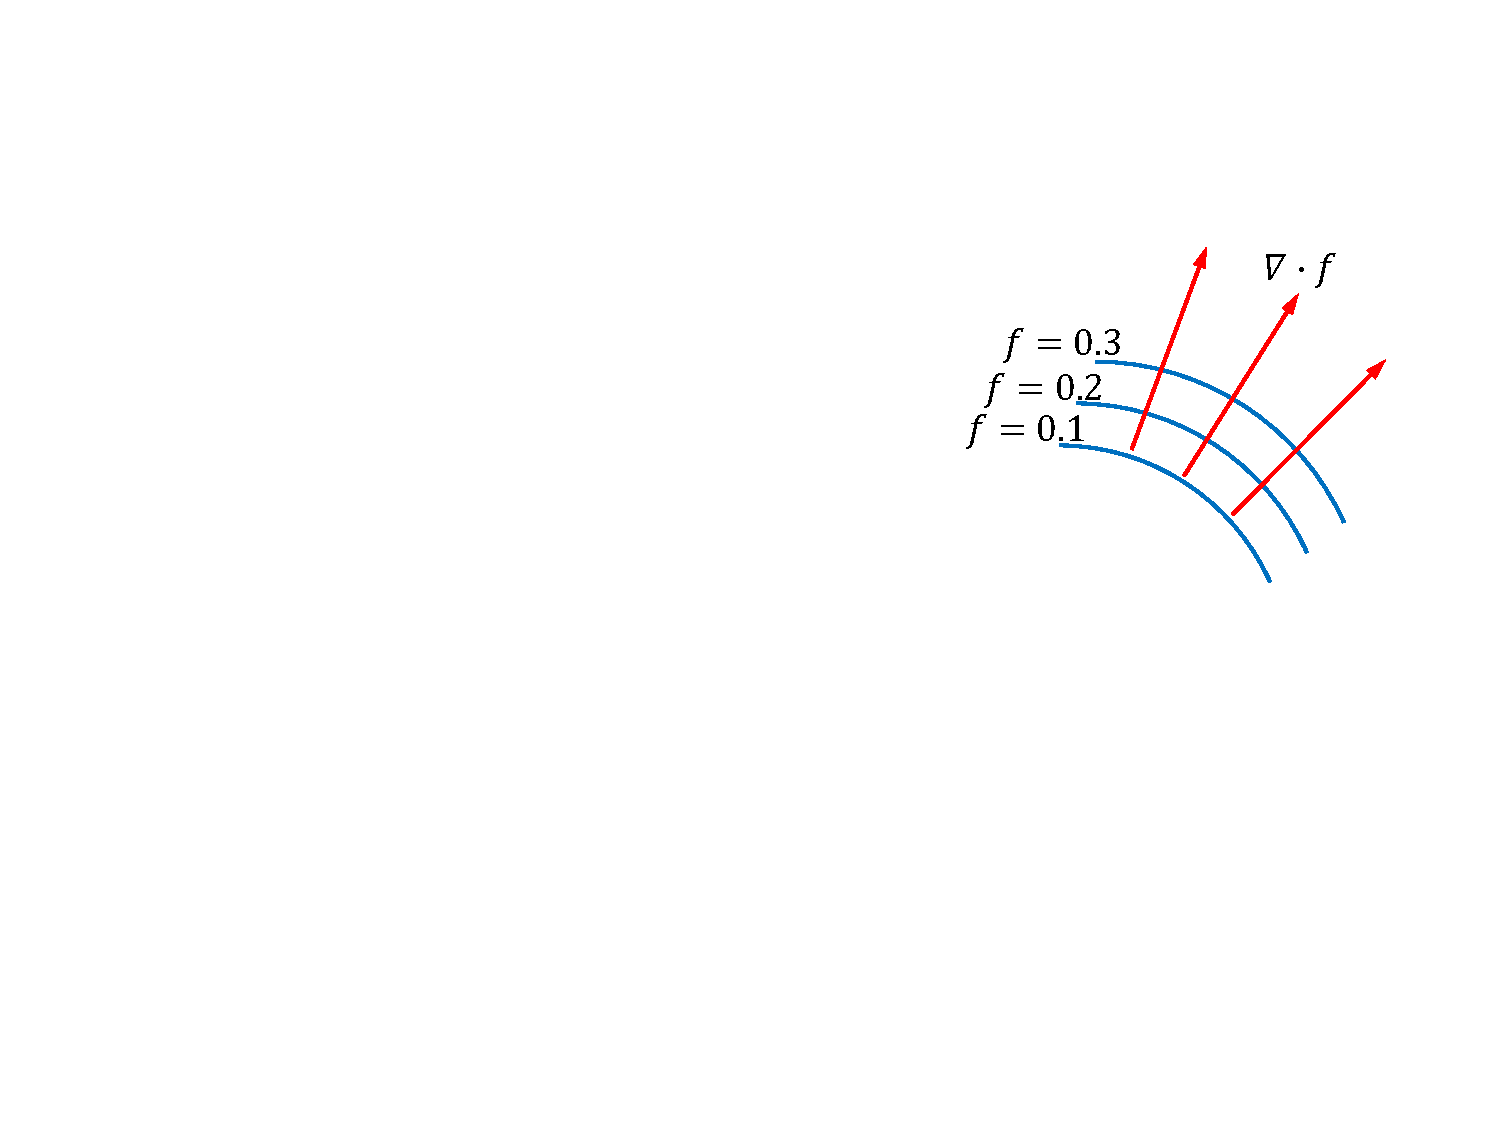
\includegraphics[width=.8\textwidth]{./images/Gradient.pdf}
\end{minipage}
\begin{minipage}[rt]{13cm}
	The gradient of a scalar field reveals the direction of the steepest ascent of the scalar function (perpendicular to the corresponding isolines of the function). \\ \\
	\begin{tabular}{ll}
		Scalar field: & \(\displaystyle f = f\left(\vec{r}\right) = f\left(x,y,z\right) \) \\ 
		Gradient is a vector: & \(\displaystyle \textrm{grad }f = \lim\limits_{\textrm{diameter}\left(D\right)\rightarrow 0} \frac{\oiint_{\textrm{boundary}\left(D\right)}f \cdot \vec{dA}}{\textrm{measure}\left(D\right)}, D\subseteq R^3 \) \\
		Gradient in Cartesian coordinates: & \(\displaystyle \textrm{grad }f = \frac{\partial f}{\partial x} \cdot \vec{e_x}+\frac{\partial f}{\partial y} \cdot \vec{e_y}+\frac{\partial f}{\partial z} \cdot \vec{e_z} \) \\ 
		$\nabla$-operator (Nabla): & \(\displaystyle \nabla = \frac{\partial}{\partial x} \cdot \vec{e_x}+\frac{\partial}{\partial y} \cdot \vec{e_y}+\frac{\partial}{\partial z} \cdot \vec{e_z} \)\\
		Gradient and $\nabla$-operator: & \(\displaystyle \textrm{grad }f = \nabla \cdot f \)\\
	\end{tabular} 
\end{minipage}

\textbf{\\ \\ Divergence\\ \\}
\begin{minipage}[lt]{5cm}
	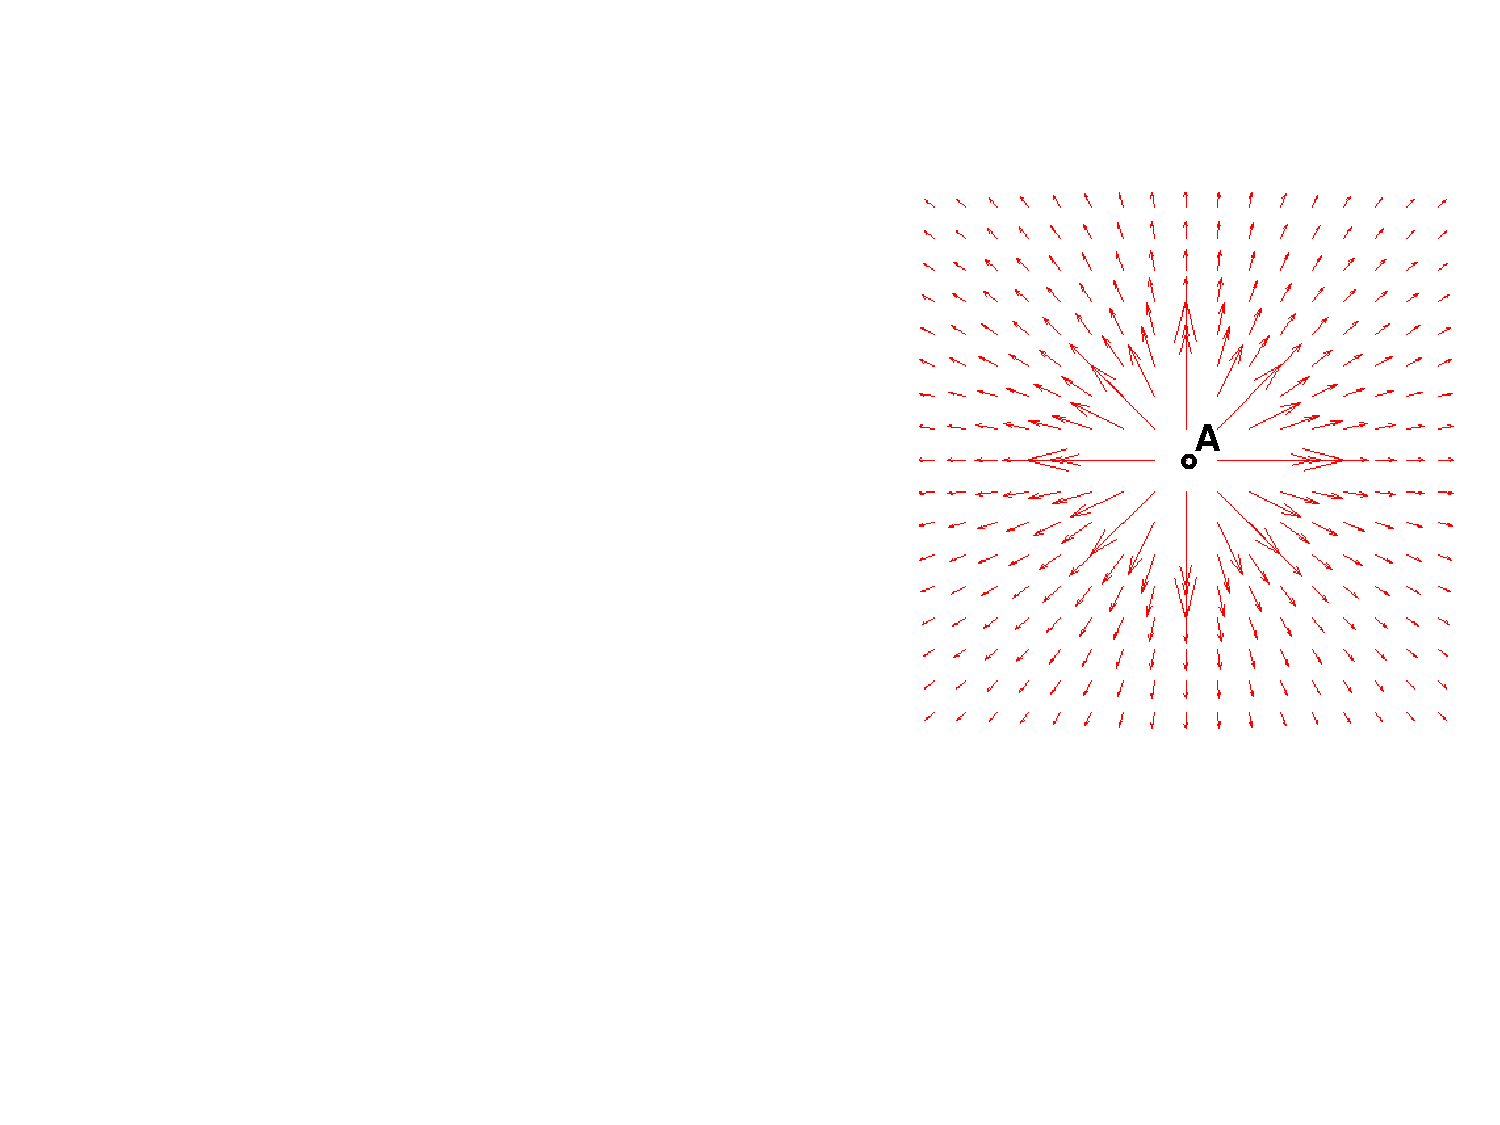
\includegraphics[width=.8\textwidth]{./images/Divergence.pdf}
\end{minipage}
\begin{minipage}[rt]{13cm}
	In the central point $A$ of this field distribution is: $\mathrm{div}~\vec{a} > 0$. Generally speaking, a positive or negative divergence reveals a field source or a field sink, respectively. \\ \\
	\begin{tabular}{ll}
		Vector field: & \(\displaystyle \vec{a} = \vec{a}\left(\vec{r}\right) = \vec{a}\left(x,y,z\right)\) \\
		Divergence is a scalar: & \(\displaystyle \mathrm{div}~\vec{a} = \lim\limits_{\textrm{diameter}\left(D\right)\rightarrow 0} \frac{\oiint_{\textrm{boundary}\left(D\right)} \vec{a} \cdot \vec{dA}}{\textrm{measure}\left(D\right)}, D\subseteq R^3\) \\
		Divergence in Cartesian coordinates: & \(\displaystyle \mathrm{div}~\vec{a} = \frac{\partial a_x}{\partial x} + \frac{\partial a_y}{\partial y} + \frac{\partial a_z}{\partial z} \)\\
		Divergence and $\nabla$-operator: & \(\displaystyle \mathrm{div}~\vec{a} = \nabla \cdot \vec{a} \) \\
	\end{tabular}
\end{minipage}

\textbf{\\ \\ Curl\\ \\}
\begin{minipage}[lt]{5cm}
	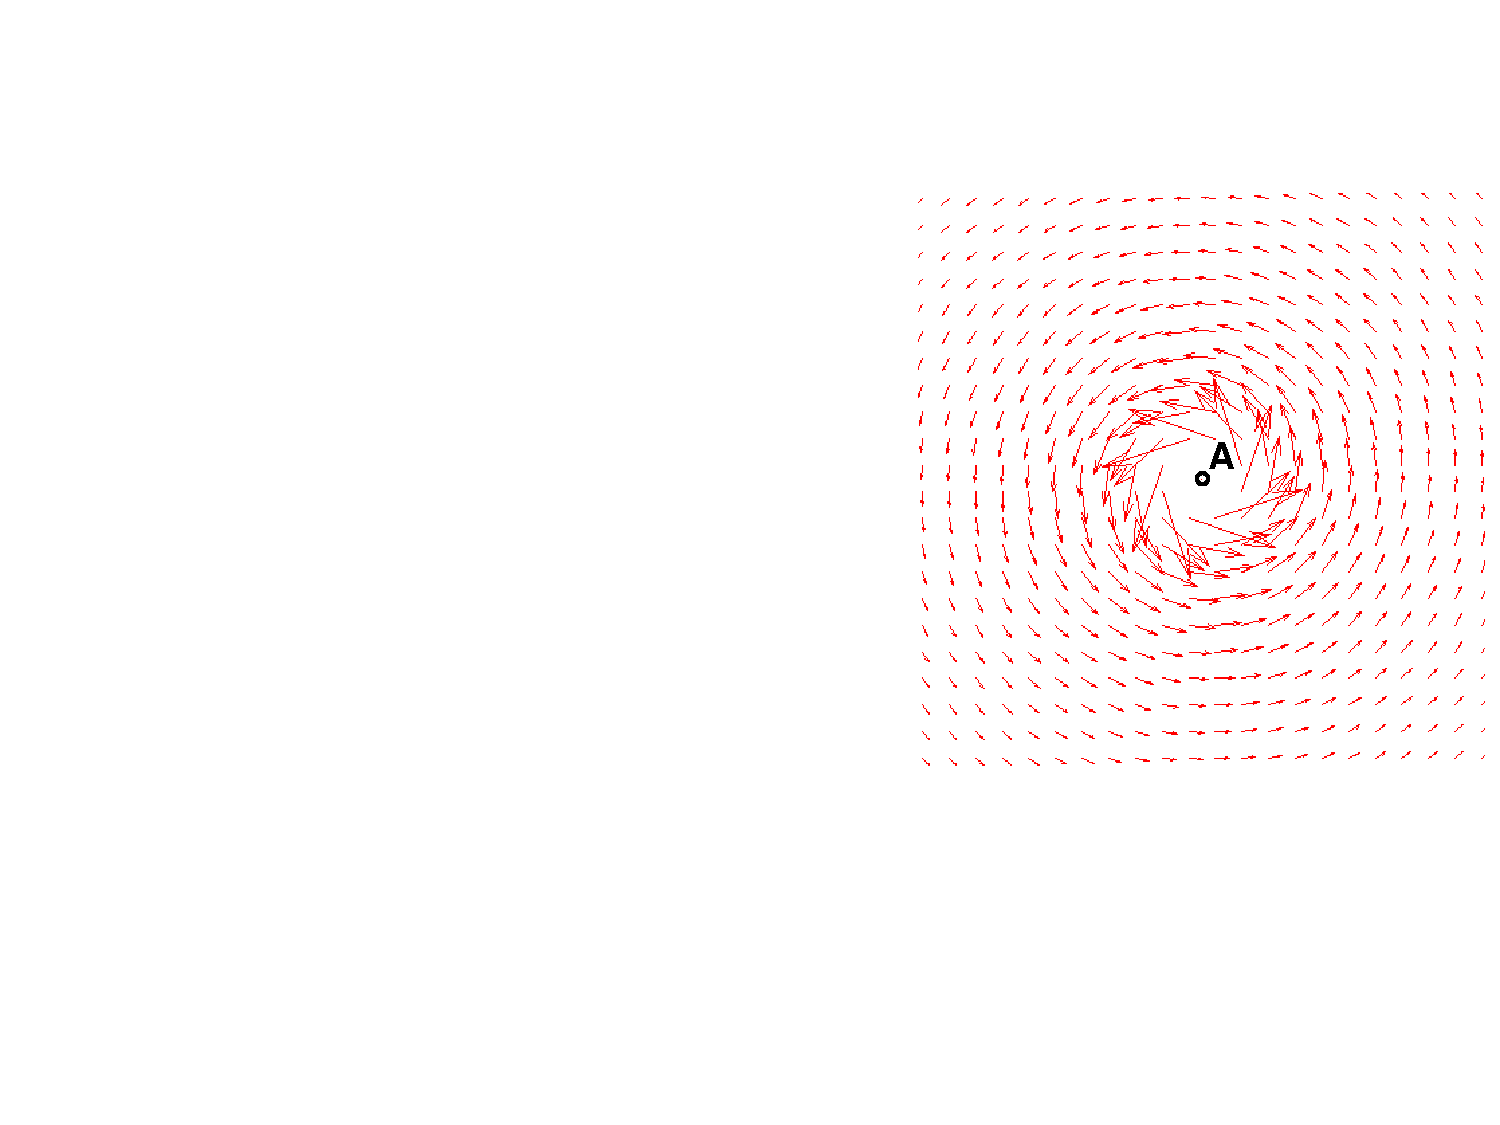
\includegraphics[width=.8\textwidth]{./images/Curl.pdf}
\end{minipage}
\begin{minipage}[rt]{13cm}
	In the central point $A$ of this field distribution is: $\textrm{curl}~\vec{a} > 0$. Generally speaking non-zero curl reveals a rotational field character. (Curl looks what stays in this area).\\ \\
	\begin{tabular}{ll}
		Vector field: & \(\displaystyle \vec{a} = \vec{a}\left(\vec{r}\right) = \vec{a}\left(x,y,z\right)\)\\
		Curl is a vector: & \(\displaystyle \textrm{curl }\vec{a} = \lim\limits_{\textrm{diameter}\left(D\right)\rightarrow 0} \frac{\oiint_{\textrm{boundary}\left(D\right)} \vec{dA} \times \vec{a}}{\textrm{measure}\left(D\right)}, D\subseteq R^3\)\\
		Curl in Cartesian coordinates: & \(\displaystyle \textrm{curl }\vec{a} = 
		\begin{vmatrix}
			\vec{e_x} & \vec{e_y} & \vec{e_z} \\
			\frac{\partial}{\partial x} & \frac{\partial}{\partial y} & \frac{\partial}{\partial z} \\
			a_x & a_y & a_z \\
		\end{vmatrix}\) \\
		Curl in Cylindrical Coordinates: & \(\displaystyle \textrm{curl }\vec{a} = \frac{1}{r} 
		\begin{vmatrix}
			\vec{e_r} & r\vec{e_\varphi} & \vec{e_z} \\
			\frac{\partial}{\partial r} & \frac{\partial}{\partial \varphi} & \frac{\partial}{\partial z} \\
			a_r & ra_\varphi & a_z \\
		\end{vmatrix} \) {\tiny \texttt{other coordinates in Bronstein: P.719ff}}\\
		& \(\displaystyle = \vec{e_x}\frac{\partial}{\partial y}a_z +   		\vec{e_y}\frac{\partial}{\partial z}a_x +\vec{e_z}\frac{\partial}{\partial x}a_y - \vec{e_x}\frac{\partial}{\partial z}a_y - \vec{e_y}\frac{\partial}{\partial x}a_z - \vec{e_z}\frac{\partial}{\partial y}a_x\) \\
		Curl and $\nabla$-operator: & \(\displaystyle \textrm{curl }\vec{a} = \nabla \times \vec{a} \) \\
	\end{tabular}
\end{minipage}



\textbf{\\ \\ Theorems\\}
	Gauss theorem:
	\begin{equation*}
		\oiint\limits_{\left(\partial \Omega\right)} \vec{a} \cdot d\vec{S} = \iiint\limits_{\left(\Omega\right)} \nabla \cdot \vec{a} \cdot dV
	\end{equation*}
	Stokes theorem:
	\begin{equation*}
		\int\limits_{\left(\partial S\right)} \vec{a} \cdot d\vec{l} = \iint\limits_{\left(S\right)} \nabla \times \vec{a} \cdot d\vec{S}
	\end{equation*}
	
\textbf{\\ \\ Rules \\}
\begin{tabular}{ll}
	Curl of a gradient is always equal to zero: & \(\displaystyle \nabla \times \left(\nabla \cdot \vec{a} \right) \equiv 0\) \\
	Divergence of a curl is always equal to zero: & \(\displaystyle \nabla \cdot \left(\nabla \times \vec{a}\right) \equiv 0 \)\\ \\
	\(\displaystyle \nabla \times \nabla \times \vec{a} = \nabla \left(\nabla \cdot \vec{a}\right) - \Delta \vec{a}\) \\
	\(\displaystyle \nabla \cdot \left(\vec{a} \times \vec{b}\right) = \vec{b} \cdot \left(\nabla \times \vec{a}\right) - \vec{a} \cdot \left(\nabla \times \vec{b}\right)\) 
\end{tabular}

\textbf{\\ \\ Operators \\} 
\begin{tabular}{ll}
	Laplace Operator: & \(\displaystyle \nabla \cdot \nabla = \nabla^2 = \Delta = \frac{\partial^2}{\partial x^2}+\frac{\partial^2}{\partial y^2}+\frac{\partial^2}{\partial z^2} \) \\
\end{tabular}
\newpage
\textbf{\\ \\ Irrotationality of electrostatic field \\}
\begin{minipage}[lt]{9cm}
	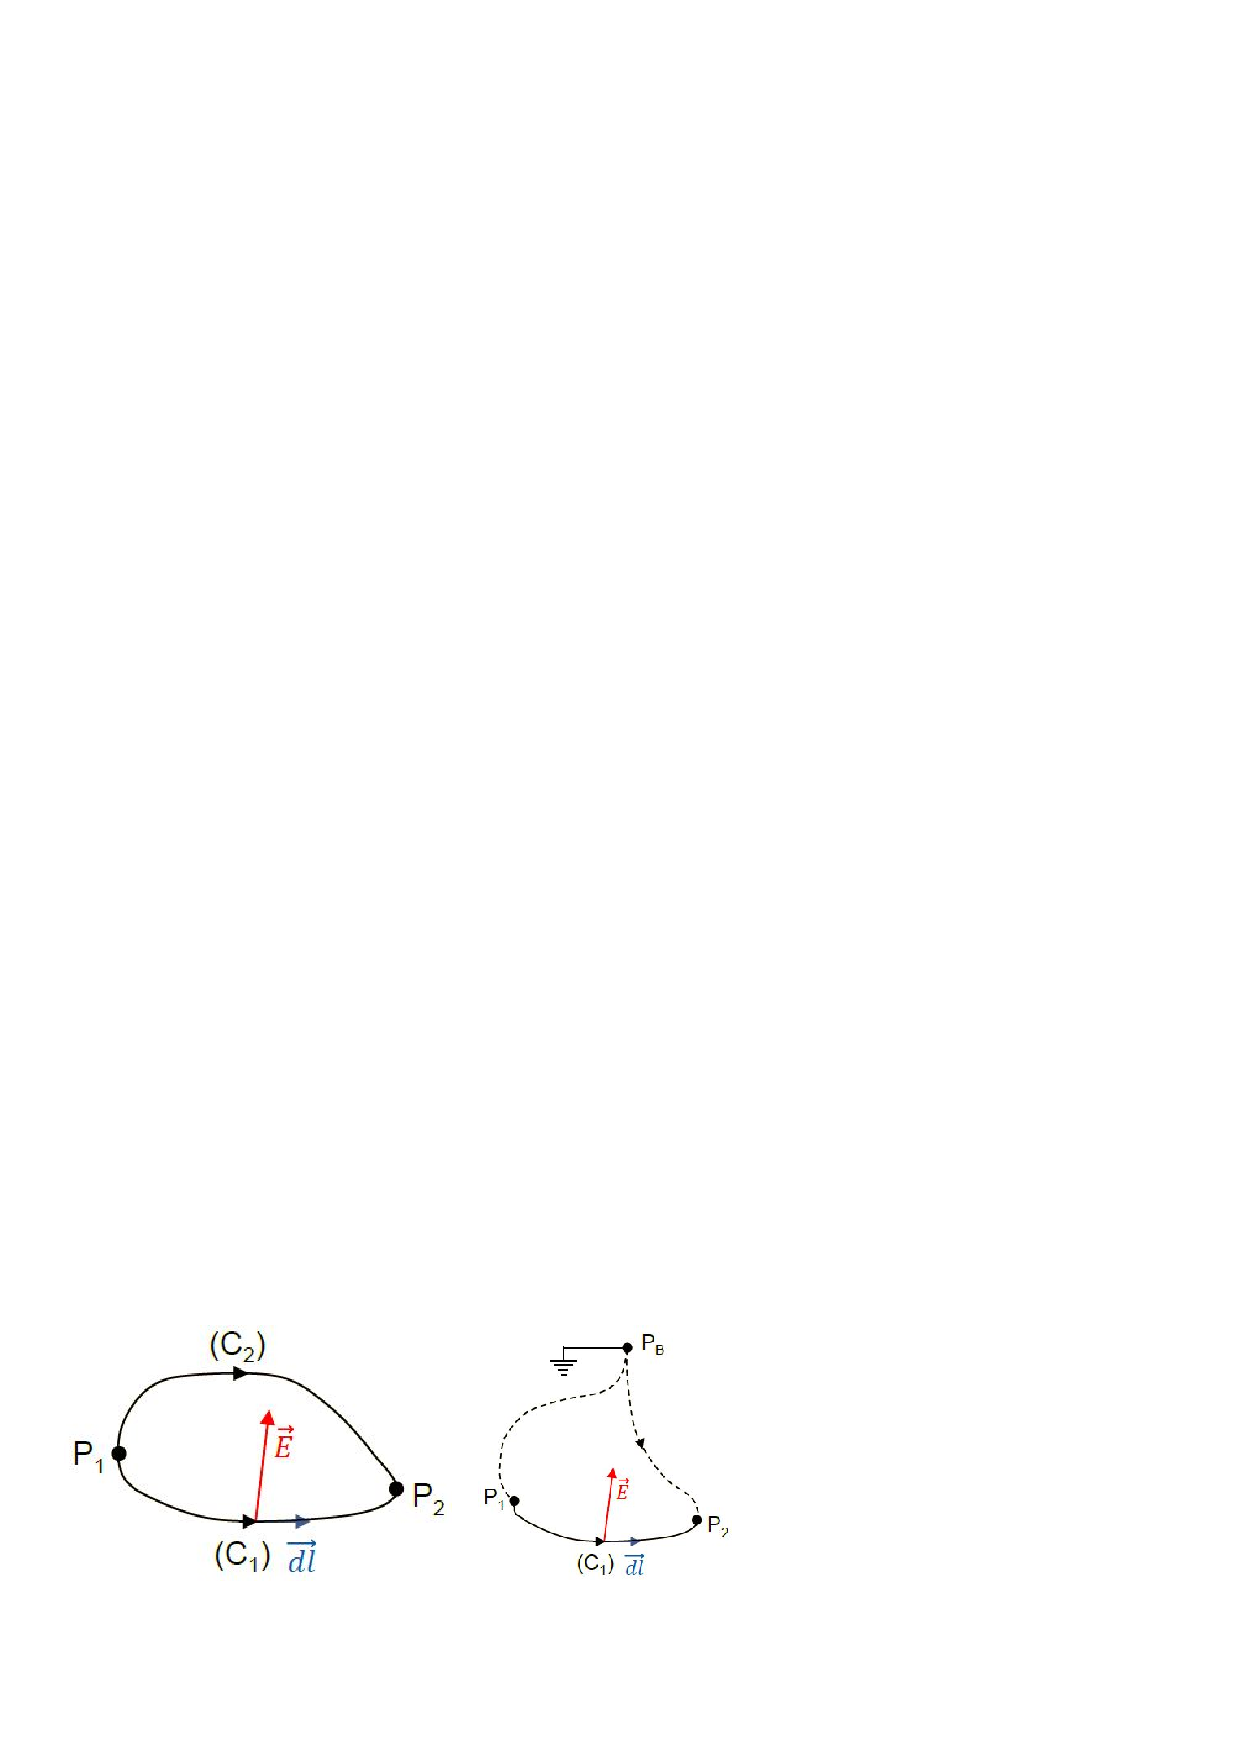
\includegraphics[width=.9\textwidth]{./images/WirbelfreiE2.pdf}
\end{minipage}
\begin{minipage}[rt]{10cm}
	\begin{equation*}
		\oint \limits_{\left(C\right)} \vec{E}\cdot \vec{dl} = 0
	\end{equation*}
	\begin{equation*}
		\int\limits_{\left(C\right)} \vec{E} \cdot \vec{dl} = \underbrace{\int_{P_1}^{P_2} \vec{E} \cdot \vec{dl}}_{C_1} - \underbrace{\int_{P_1}^{P_2} \vec{E} \cdot \vec{dl}}_{C_2} = 0
	\end{equation*}
	\begin{equation*}
		V_{P_1P_2} = \varphi_{P_1} - \varphi_{P_2} = \int_{P_1}^{P_B} \vec{E} \cdot \vec{dl} - \int_{P_1}^{P_B} \vec{E} \cdot \vec{dl} = \int_{P_1}^{P_2} \vec{E} \cdot \vec{dl}
	\end{equation*}
\end{minipage}
The line integral of an electrostatic field only depends on the start and end point. It is independent of the chosen path (conservative field).
	
\textbf{\\ \\Continuity Equation\\}
	The current through a closed oriented surface $(S)$ can be computed as
	\begin{equation*}
		I = \oiint\limits_{\left(S\right)} \vec{J} \cdot \vec{dS}
	\end{equation*}
	Because of conservation the outflowing current must be equal to the decreasing total charge in volume $(V)$.
	\begin{equation*}
		I = -\frac{dQ}{dt} = -\frac{d}{dt}\iiint\limits_{\left(V\right)} \rho \cdot dV = -\iiint\limits_{\left(V\right)} \frac{d \rho}{dt}dV
	\end{equation*}
	Both combined leads to the Continuity Equation
	\begin{equation*}
		\oiint\limits_{\left(S\right)} \vec{J} \cdot \vec{dS} = - \iiint\limits_{\left(V\right)} \frac{d\rho}{dt}dV \rightarrow \nabla \cdot \vec{J} = -\frac{\partial \rho}{\partial t}
	\end{equation*}

\textbf{\\ Ohmic law\\}
\begin{minipage}[lt]{11cm}
	\begin{tabular}{l}
		\(\displaystyle dI = \frac{dU}{R} = G \cdot dU = \sigma \cdot \frac{dA}{l} \cdot dU \) \\
		\(\displaystyle G = \sigma \cdot \frac{dA}{l} \hspace{2cm} R = \rho \cdot \frac{l}{s} \) \\
		\(\displaystyle J \cdot dA = \sigma \cdot \frac{dA}{l} \cdot E \cdot l \rightarrow J = \sigma \cdot E \) \\
		or as vectors: \(\displaystyle \vec{J} = \sigma \cdot \vec{E}\)
	\end{tabular}
\end{minipage}
\begin{minipage}[rt]{8cm}
	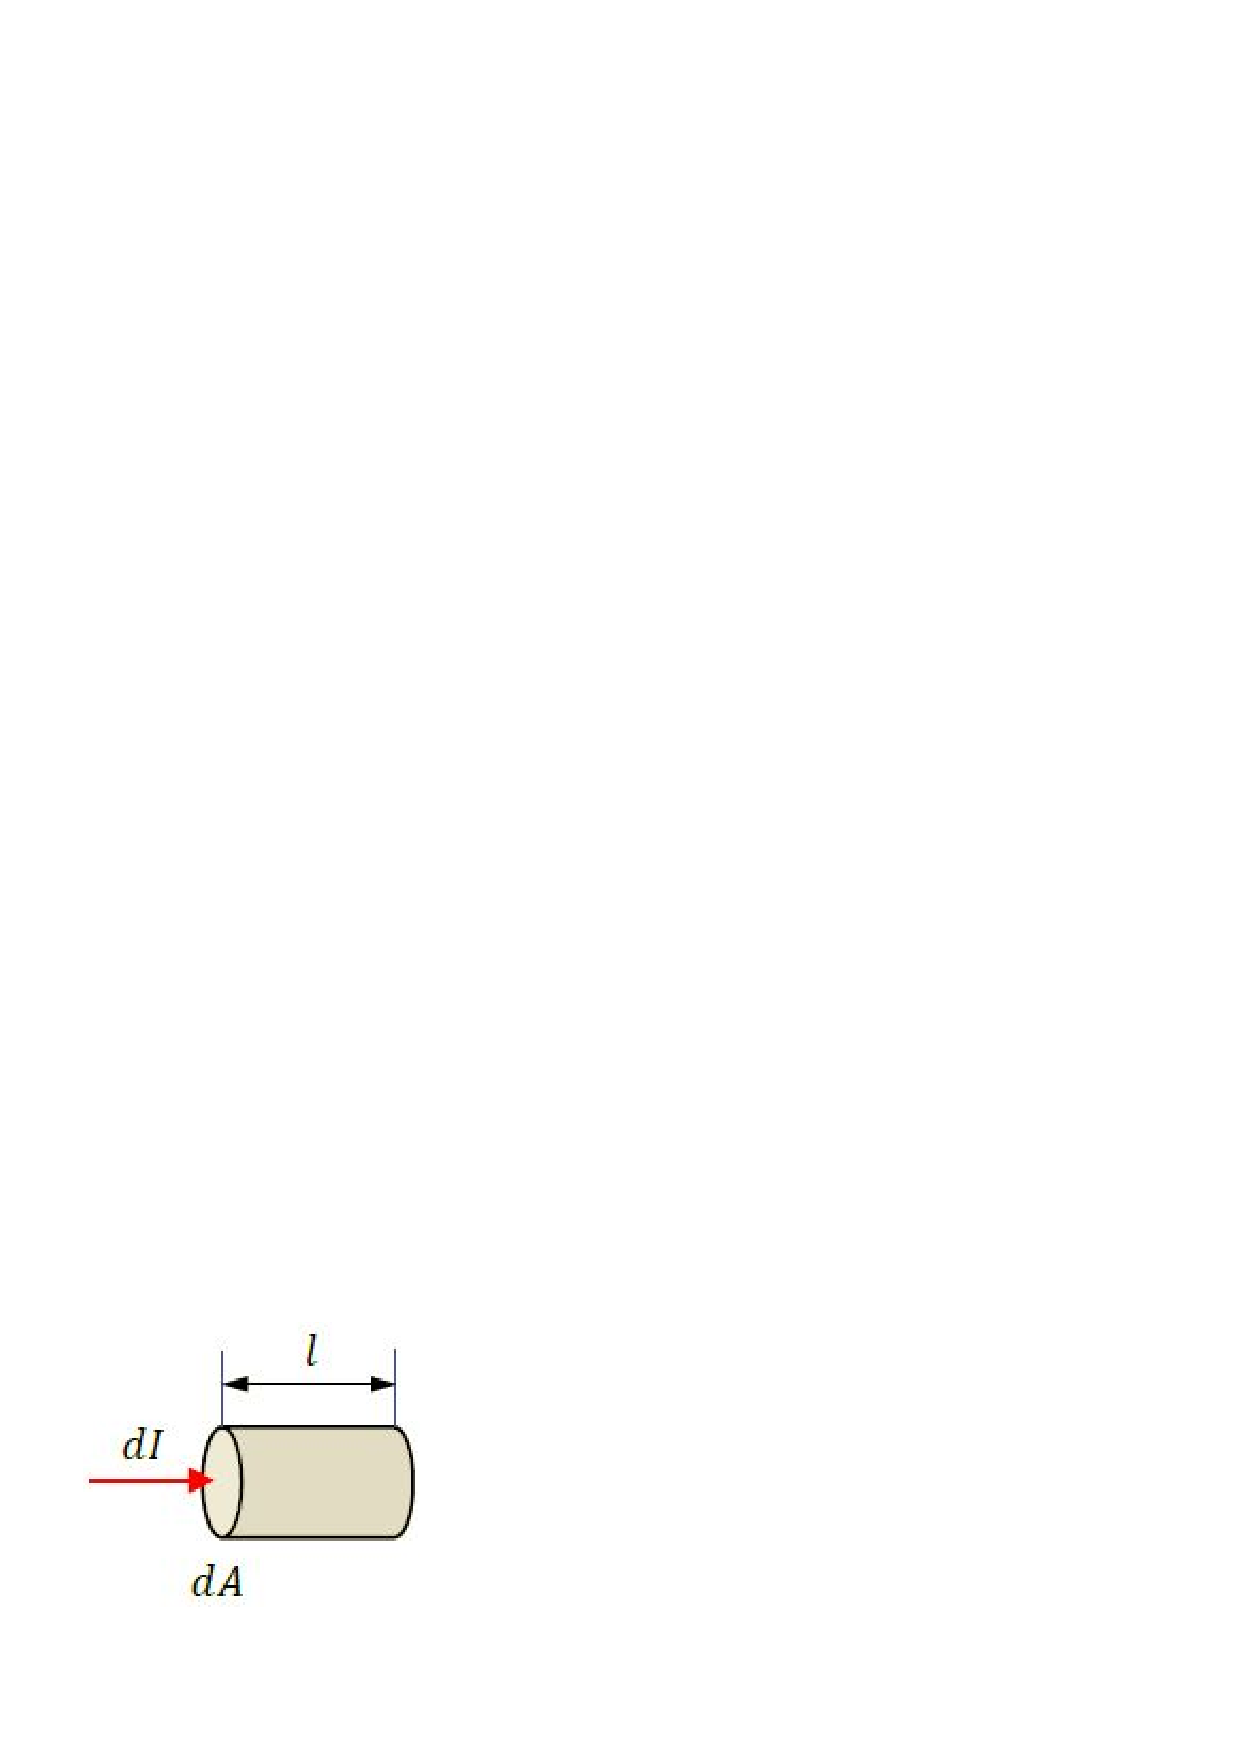
\includegraphics[width=.5\textwidth]{./images/ohmic.pdf}
\end{minipage}

\textbf{\\ \\ Skin effect\\}
\begin{tabular}{ll}
	Skin depth (where it is $e$-times lower) $[m]$: & \(\displaystyle \delta = \sqrt{\frac{2}{\omega \mu_0\sigma}} \) \\
	Skin depth for cupper at $50~Hz$: & \(\displaystyle \delta_{Cu} \approx 9mm \)
\end{tabular}


\section{Maxwell Equations}

\subsection{Integral form}
\begin{multicols}{2}
	\textbf{Gauss's law, 1835\newline}
	\noindent The electric flux density $\vec{D} = \varepsilon \vec{E}$ through a closed oriented area $(A)$ is equal to the total electric charge $Q$ which is surrounded by this area.
	\begin{equation}
		\oiint\limits_{\left(\partial\Omega\right)} \vec{D}\left(\vec{r}\right)\cdot d\vec{S}\left(\vec{r}\right) = Q = \iiint\limits_{\left(\Omega\right)}\rho\left(\vec{r}\right)\cdot dV\left(\vec{r}\right)
		\label{eq:MaxwellInt1}
	\end{equation}
	
	\textbf{Coulomb's law, 1785\newline}
	\noindent The magnetic flux trough a closed oriented area is alway zero! This means there are no magnetic monopols.
	\begin{equation}
		\oiint\limits_{\left(\partial\Omega\right)} \vec{B}\left(\vec{r}\right)\cdot d\vec{S}\left(\vec{r}\right) = 0
		\label{eq:MaxwellInt2}
	\end{equation}
	
	\textbf{Ampère's law, 1826\newline}
	The sum of all currents through a closed oriented area can be computed as
	\begin{equation}
		\oint\limits_{\left(\partial S\right)} \vec{H}\left(\vec{r}\right)\cdot d\vec{l}\left(\vec{r}\right) = \sum_{k=1}^{N} I_k = \Theta =  \iint\limits_{\left(S\right)}\vec{J}\left(\vec{r}\right)\cdot d\vec{S}\left(\vec{r}\right)
		\label{eq:MaxwellInt3}
	\end{equation}
	
	\textbf{Faraday's law, 1831\newline}
	A time-dependent magnetic flux induces an electrical voltage.
	\begin{equation}
		u_i = \oint\limits_{\left(\partial S\right)} \vec{E}\left(\vec{r}\right)\cdot d\vec{l}\left(\vec{r}\right) = -\frac{\partial \Phi}{\partial t} = -\frac{\partial}{\partial t} \iint\limits_{\left(S\right)} \vec{B}\left(\vec{r}\right)\cdot d\vec{S}\left(\vec{r}\right)
		\label{eq:MaxwellInt4} 
	\end{equation}
\end{multicols}

\begin{figure}[h!]
	\centering
	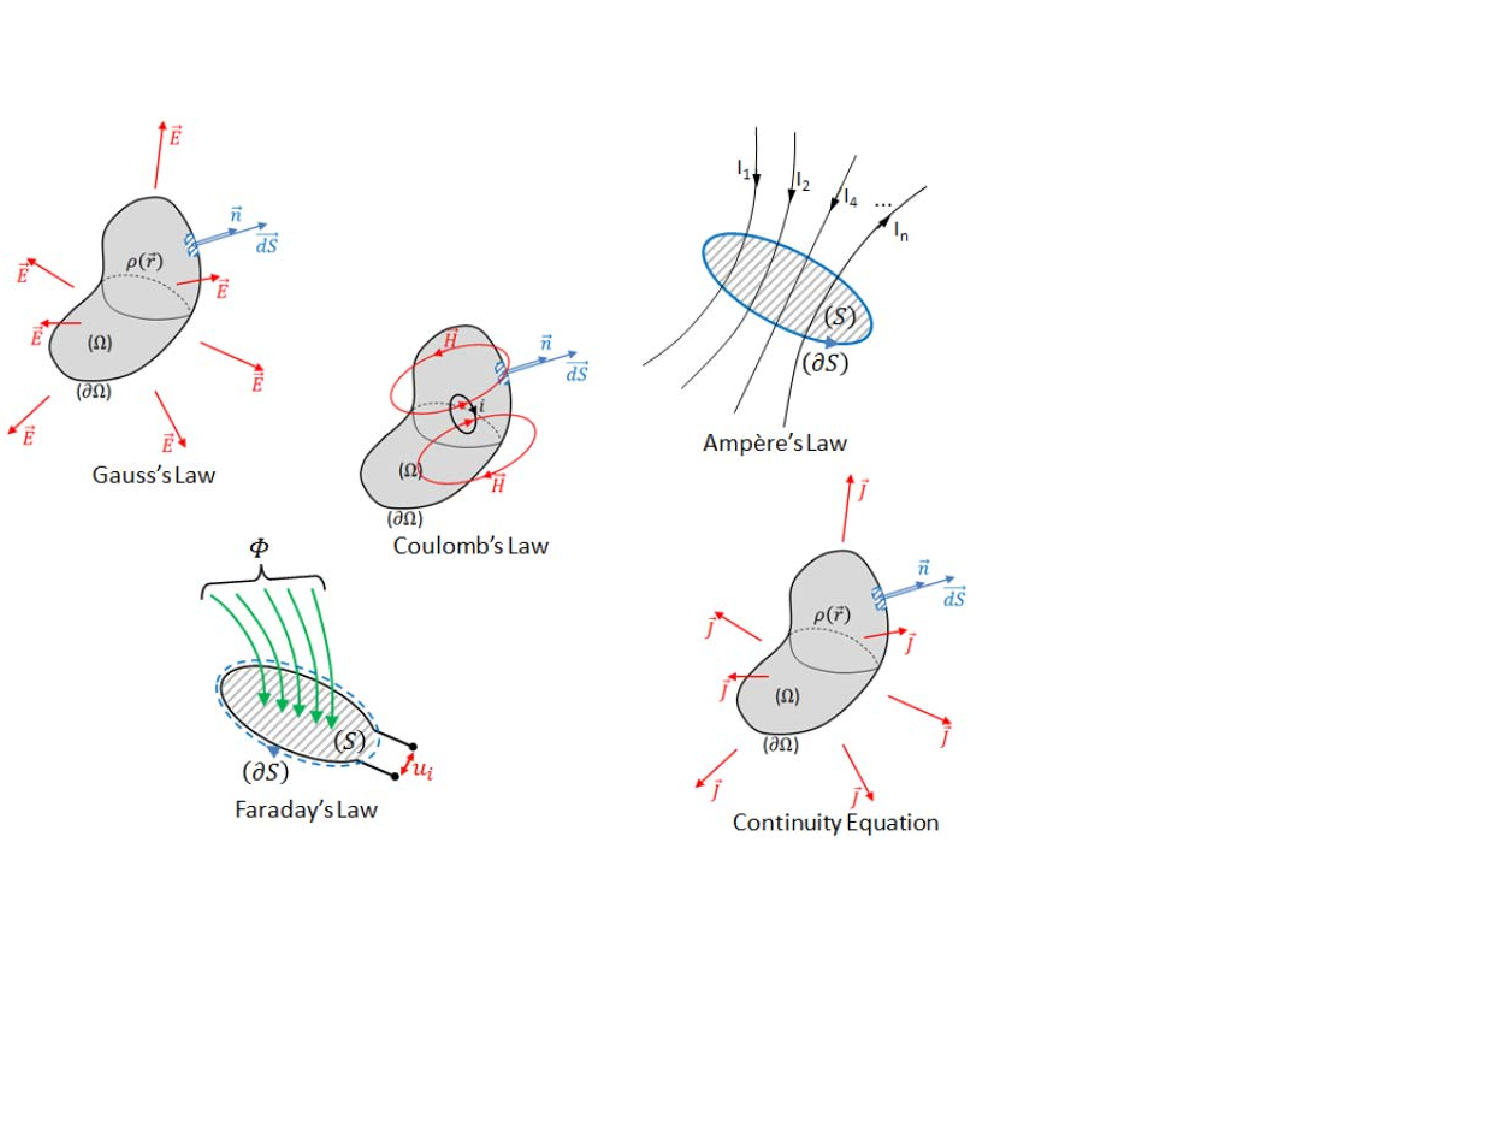
\includegraphics[width=.55\textwidth]{./images/MaxwellEqImages.pdf}
\end{figure}

\subsection{Maxwell Equations in time domain}
Using Gauss Theorem on Equation (\ref{eq:MaxwellInt1}) and (\ref{eq:MaxwellInt2}) and Stokes Theorem on (\ref{eq:MaxwellInt3}) and (\ref{eq:MaxwellInt4}) the following Maxwell Equations in time domain can be obtained as 
\begin{multicols}{2}
	\begin{equation}
		\nabla \cdot \vec{D} = \rho
		\label{eq:MaxwellDiff1_1}
	\end{equation}
	\begin{equation}
		\nabla \cdot \vec{B} = 0
		\label{eq:MaxwellDiff1_2}
	\end{equation}
	\begin{equation}
		\nabla \times \vec{H} = \vec{J} + \frac{\partial \vec{D}}{\partial t} = \sigma \vec{E} + \varepsilon \frac{\partial \vec{E}}{\partial t}
		\label{eq:MaxwellDiff1_3}
	\end{equation}
	\begin{equation}
		\nabla \times \vec{E} = - \frac{\partial \vec{B}}{\partial t}
		\label{eq:MaxwellDiff1_4}
	\end{equation}
	
	\begin{equation}
		\nabla \cdot \vec{E} = \frac{\rho}{\varepsilon}
		\label{eq:MaxwellDiff2_1}
	\end{equation}
	\begin{equation}
		\nabla \cdot \vec{H} = 0
		\label{eq:MaxwellDiff2_2}
	\end{equation}
	\begin{equation}
		\nabla \times \vec{B} = \mu\left(\vec{J} + \frac{\partial \vec{D}}{\partial t}\right)
		\label{eq:MaxwellDiff2_3}
	\end{equation}
	\begin{equation}
		\nabla \times \vec{E} = -\mu \frac{\partial \vec{H}}{\partial t}
		\label{eq:MaxwellDiff2_4}
	\end{equation}
\end{multicols}
where Equation (\ref{eq:MaxwellDiff1_3}) and (\ref{eq:MaxwellDiff2_3}) show $\vec{H} \rightarrow \vec{E}$ coupling and Equation (\ref{eq:MaxwellDiff1_4}) and (\ref{eq:MaxwellDiff2_4}) show $\vec{E} \rightarrow \vec{H}$ coupling.

\subsection{Maxwell Equations in frequency domain}
If the field sources are harmonic sinusoidal time functions, the fields must have also this time dependence if the involved materials are linear. The fields can be represented as the following complex vectors
\begin{equation*}
	\vec{F}\left(\vec{r},t\right) = \Re\{\underline{\vec{F}}\left(\vec{r}\right) \cdot e^{j\omega t}\}.
\end{equation*}
The main advantage of this approach is the following elimination of the time derivatives
\begin{equation*}
	\frac{\partial}{\partial t}\left(e{j \omega t}\right) = j \omega^\cdot e^{j \omega t}
\end{equation*}
applied to the Maxwell Equations in time domain the following is obtained
\begin{equation*}
	\nabla \cdot \underline{\vec{D}}\left(\vec{r}\right) = \underline{\rho}\left(\vec{r}\right)
\end{equation*}
\begin{equation*}
	\nabla \cdot \underline{\vec{B}}\left(\vec{r}\right) = 0
\end{equation*}
\begin{equation*}
	\nabla \times \underline{\vec{H}}\left(\vec{r}\right) = \underline{\vec{J}}\left(\vec{r}\right) + j \omega \cdot \underline{\vec{D}}\left(\vec{r}\right)
\end{equation*}
\begin{equation*}
	\nabla \times \underline{\vec{E}}\left(\vec{r}\right) = - j\omega \underline{\vec{B}}\left(\vec{r}\right)
\end{equation*}
\section{Electrostatic Analysis}

The electric and magnetic fields are completely decoupled (the field induction cease to exist). E-field and H-field exist independent from each other. \\

Since $\frac{\partial}{\partial t} = 0$, Maxwell Equations (\ref{eq:MaxwellDiff1_1}), (\ref{eq:MaxwellDiff1_4}), (\ref{eq:MaxwellDiff2_1}) and (\ref{eq:MaxwellDiff2_4}) can be written as

\begin{tabular}{ll}
	\(\displaystyle \nabla \cdot \vec{D} = \rho \) & \(\displaystyle \nabla \cdot \vec{E} = \frac{\rho}{\varepsilon} \) \\
	\(\displaystyle \nabla \times \vec{E} = 0 \) \hspace{2cm} & \(\displaystyle \nabla \times \vec{E} = 0 \) .
\end{tabular}

Since the curl of the electric field is always equal to zero, the electric field can be described as agradient of the electric scalar potential
\begin{equation*}
	\vec{E} = -\nabla \varphi \rightarrow \underbrace{\nabla \cdot \left(\varepsilon \nabla \varphi\right) = -\rho}_{\text{quasi-Poisson equation}} \rightarrow \nabla \cdot \nabla \varphi = -\frac{\rho}{\varepsilon} \rightarrow \underbrace{\Delta \varphi = -\frac{\rho}{\varepsilon}}_{\text{Poisson equation if $\varepsilon$ is everywhere equal}}
\end{equation*}
Thus, in a homogeous material the electric field is a solution of the following Poisson
\begin{equation*}
	\frac{\partial^2 \varphi}{\partial x^2} + \frac{\partial^2 \varphi}{\partial y^2} +\frac{\partial^2 \varphi}{\partial z^2} = \Delta \varphi = - \frac{\rho}{\varepsilon}
\end{equation*}
or the following Laplace equation
\begin{equation*}
	\frac{\partial^2 \varphi}{\partial x^2} + \frac{\partial^2 \varphi}{\partial y^2} +\frac{\partial^2 \varphi}{\partial z^2} = \Delta \varphi = 0
\end{equation*}
written in Cartesian coordinate. {\tiny \texttt{other coordinates in Bronstein: P.723}}

\textbf{\\ Boundary Value Problem (BVP)\\}
\begin{minipage}[lt]{11cm}
	\begin{tabular}{l}
		\(\displaystyle \frac{\partial^2 \varphi}{\partial x^2} + \frac{\partial^2 \varphi}{\partial y^2} +\frac{\partial^2 \varphi}{\partial z^2} = \Delta \varphi = - \frac{\rho}{\varepsilon}, \textrm{ in } \Omega\) \\
		\(\displaystyle \varphi = 0, \textrm{ over } \partial_{D2} \Omega \) \\
		\(\displaystyle \varphi = U, \textrm{ over } \partial_{D1} \Omega \rightarrow \) Dirichlet Boundary \\
		\(\displaystyle \frac{\partial \varphi}{\partial n} = 0, \textrm{ over } \partial_{N} \Omega \rightarrow \) Neumann Boundary \\	
		Definition Normalenableitung: \(\displaystyle \vec{n} \cdot \left(\nabla \varphi\right) = \frac{\partial \varphi}{\partial n}\)	
	\end{tabular}
\end{minipage}
\begin{minipage}[rt]{8cm}
	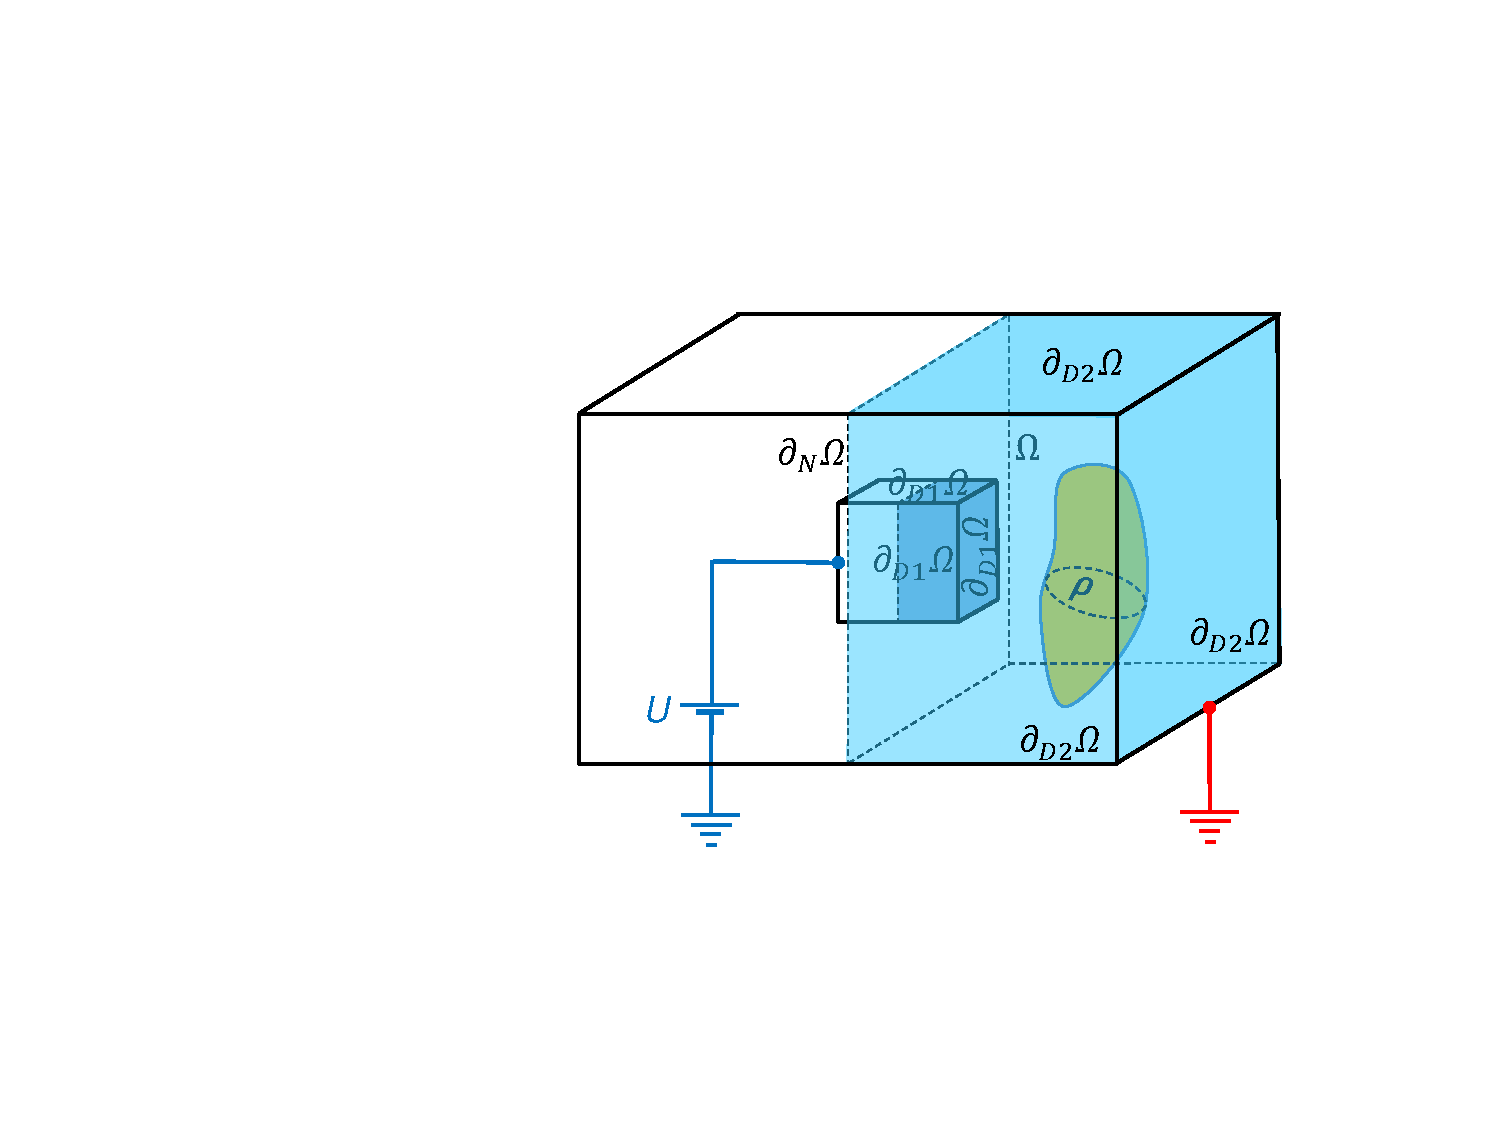
\includegraphics[width=.8\textwidth]{./images/BVP_electrostatic.pdf}
\end{minipage}
\section{Magnetostatic Analysis}

\textbf{Magnetic vector potential \\ \\}
In case when the electric field does not depend on time the following can be written
\begin{equation*}
	\nabla \cdot \vec{B} = 0
\end{equation*}
\begin{equation*}
	\nabla \times \vec{H} = \vec{J}
\end{equation*}
Due to the fact that a divergence of a curl is always equal to zero, it is possible in this case to represent the magnetic flux density as a curl of a vector function 
\begin{equation*}
	\vec{B} = \nabla \times \vec{A}
\end{equation*}
which is called the magnetic vector potential. It must fulfil the following partial differential equation
\begin{equation*}
	\underbrace{\underbrace{\nabla \times \left(\frac{1}{\mu}\underbrace{\nabla \times \vec{A}}_{\bot}\right)}_{\bot} = \vec{J}}_{||}
\end{equation*}
If the material is homogeneous, the last equation could be further simplified as 
\begin{equation*}
	\Delta\vec{A} = -\mu \vec{J}
\end{equation*}

\textbf{\\ Boundary Value Problem (BVP)\\}
\begin{minipage}[lt]{11cm}
	\begin{tabular}{l}
		\textbf{3D:} \\
		\(\displaystyle \nabla \times \left(\frac{1}{\mu}\nabla \times \vec{A}\right) = \vec{J} \) \\
		\(\displaystyle \vec{n} \times \vec{A} = 0, \textrm{ over } \partial_D\Omega \) \\
		\(\displaystyle \vec{n} \times \nabla \times \vec{A} = 0,\textrm{ over } \partial_N\Omega \) \\
		\textbf{2D planar (from book):} \\
		\(\displaystyle -\frac{\partial }{\partial x} \left(\frac{1}{\mu} \frac{\partial A_z}{\partial x}\right) - \frac{\partial }{\partial y} \left(\frac{1}{\mu} \frac{\partial A_z}{\partial y}\right) = J_z \) \\
		\(\displaystyle A_z = 0, \textrm{ over } \partial_D\Omega \) \\
		\(\displaystyle \frac{\partial A_z}{\partial n} = 0, \textrm{ over } \partial_N\Omega\) \\
		\textbf{First, the current density $\vec{J}$ must be computed to obtain a magnetostatic solution.}
	\end{tabular}
\end{minipage}
\begin{minipage}[rt]{8cm}
	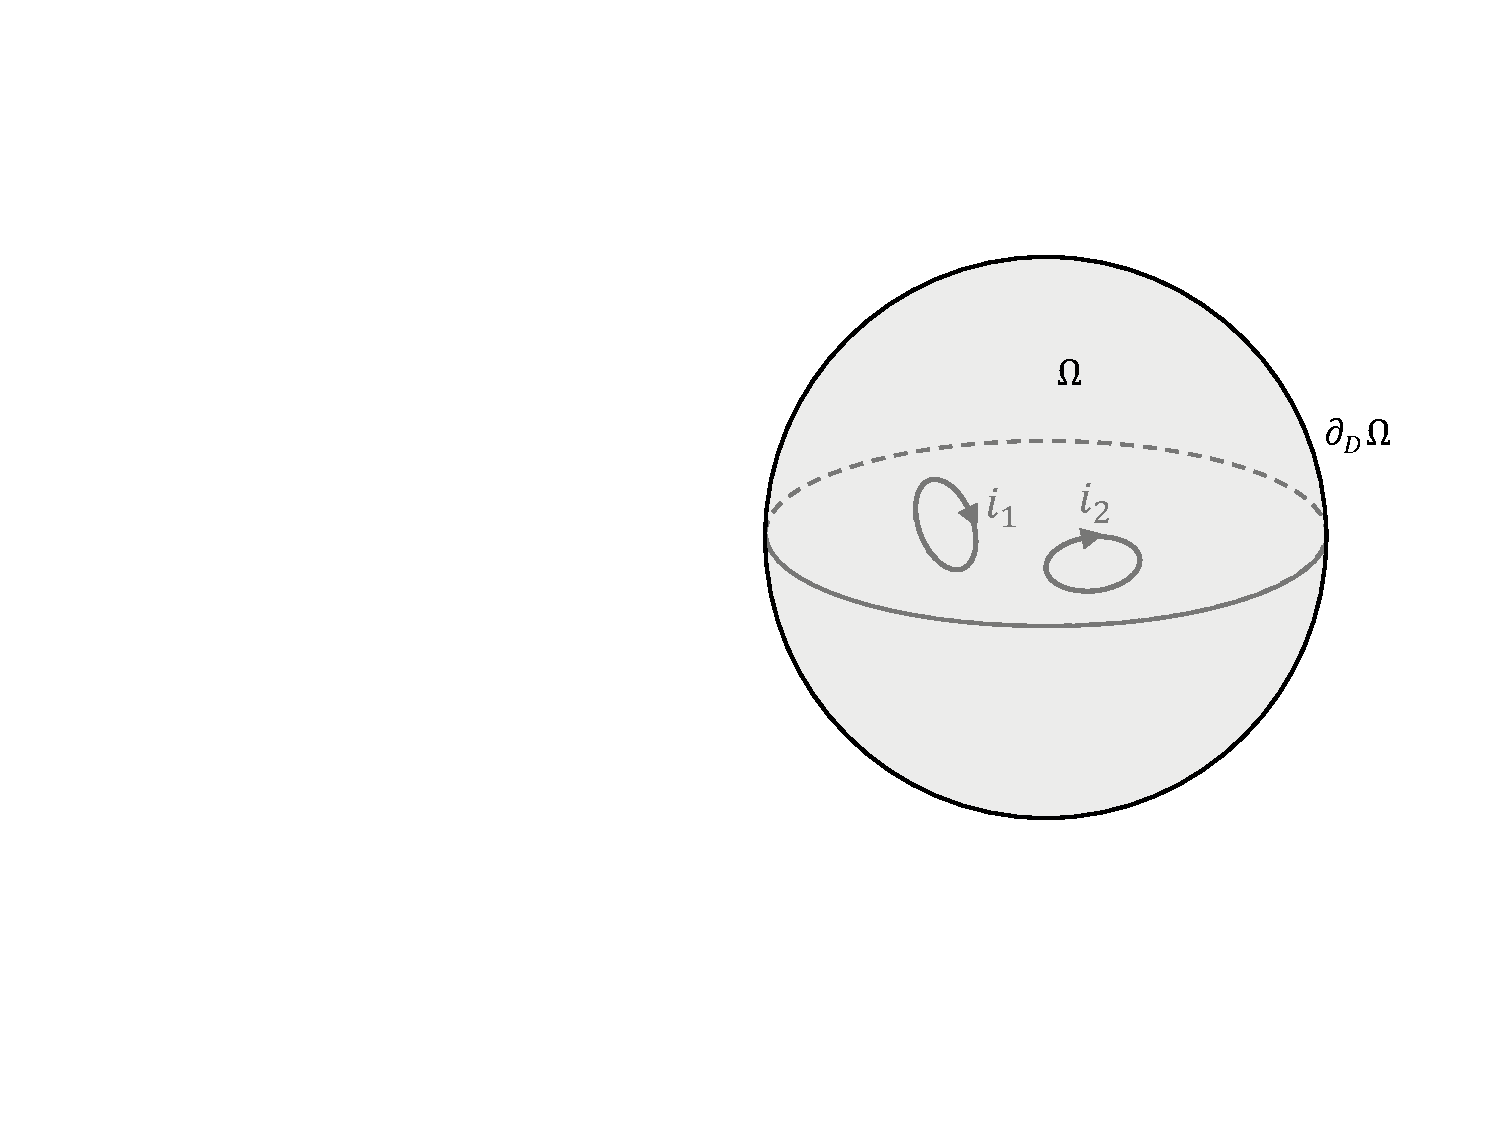
\includegraphics[width=.8\textwidth]{./images/BVP_magnetostatic.pdf}
\end{minipage}

\textbf{\\ \\ Post processing \\ }
\begin{tabular}{ll}
	Magnetic energy $\left[Ws\right]$: & \(\displaystyle W_m = \frac{1}{2} \iiint\limits_{\left(\Omega\right)} \vec{B} \cdot \vec{H} dV \) \\
	Inductivity $\left[H\right]$: & \(\displaystyle \frac{2 W_m}{I^2} \) 
\end{tabular}
\section{Boundary Conditions (BC)}
\subsection{Interface Conditions}
\begin{minipage}[rt]{8cm}
	\begin{tabular}{l}
		\(\displaystyle \left(\vec{D}_1 - \vec{D}_2\right) \cdot \vec{n} = \rho_S\) \\
		\(\displaystyle\left(\vec{B}_1 - \vec{B}_2\right) \cdot \vec{n} = 0\)\\
		\(\displaystyle\left(\vec{H}_2 - \vec{H}_1\right) \times \vec{n} =\vec{J}_S\) \\
		\(\displaystyle\left(\vec{E}_2 - \vec{E}_1\right) \times \vec{n} = 0\)\\
	\end{tabular}
\end{minipage}
\begin{minipage}[lt]{11cm}
	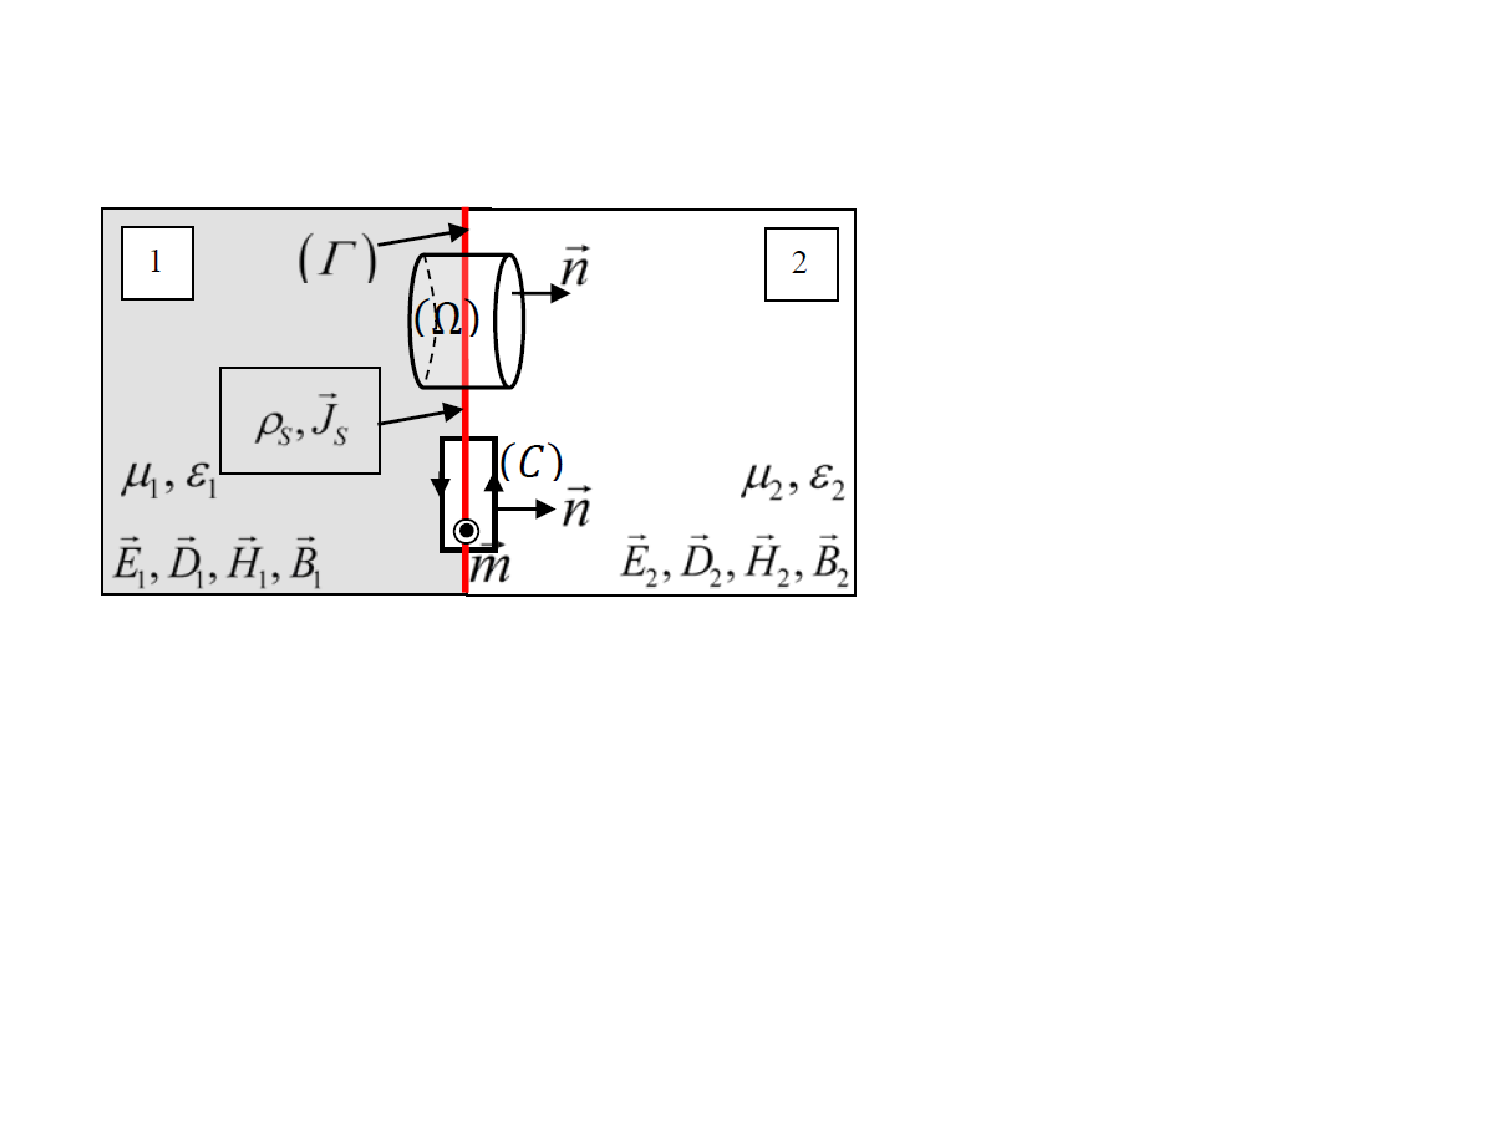
\includegraphics[width=.6\textwidth]{./images/InterfaceConditions.pdf}\\
\end{minipage}
The above interface conditions show the field behavior over the border between two different materials. \newline
The normal flux density continuity conditions can be derived by integrating Equations (\ref{eq:MaxwellInt1}) and (\ref{eq:MaxwellInt2}) over the cylinder $\Omega$ depicted above. \newline
The tangential field continuity conditions can be proven by integrating Equations (\ref{eq:MaxwellInt3}) and (\ref{eq:MaxwellInt4}) along the contour $C$ shown above.

\end{document}
